% Chapter Template

\chapter{Evaluation} % Main chapter title

\label{Chapter7} % Change X to a consecutive number; for referencing this chapter elsewhere, use \ref{ChapterX}

TODO review the core goals outlined in the introduction, and methodically review how well my final prototypes stack up against those goals. This section serves to prove (with all the data) that the approach I've described in the previous chapters actually works.

TODO a huge portion of this chapter can come from the "Interesting Graphs for my Thesis" document.


\section{Compatibility with Standard Speedcubes}

TODO discuss how well my design meets this requirement from the Introduction

The design must be deployable within a standard (non-smart) speedcube.
\begin{enumerate} 
    \item The design must not require permanent modifications to the original speedcube.
    \item The design must not significantly impact the turn-speed of the original speedcube.
\end{enumerate}


\section{Move Tracking Accuracy}

TODO discuss how well my design meets this requirement from the Introduction

The design must be capable of tracking the face turns of a Rubik's Cube with over 99\% accuracy.

This is the section for all the graphs from my "Interesting Graphs for Thesis" word document.

\begin{figure}[h]
    \centering
    \caption{Effect of stdv multiplier on accuracy of detection by cube}
    \label{fig:similarity-by-cube}
    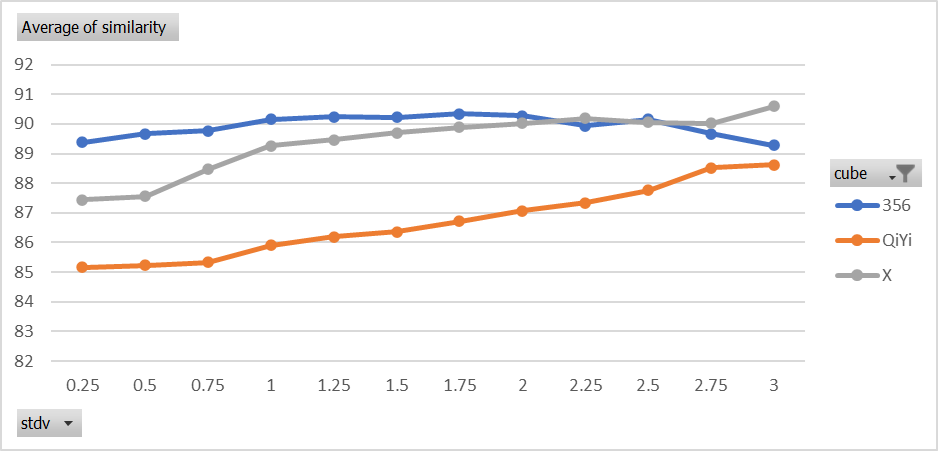
\includegraphics[width=0.75\linewidth]{Figures/7 Evaluation/similarity_by_cube.png}
\end{figure}

The 356 is the quietest cube which means its use does not add much
noise to the signal. As a result, it is not surprising that it performs
well with a low stdv multiplier. What is surprising is the degradation
of accuracy after reaching a multiplier of 2.

The QiYi is the noisiest of the three which explains its poor
performance with low multipliers. It is interesting that its accuracy
rises consistently with an increase in the stdv multiplier, although we
can see a slight taper in the rate of increase in the shift from 2.75
to 3. It would also be interesting to see how the QiYi performs at
higher multipliers (e.g. 4, 5 or higher).

The X is also a fairly noisy cube which explains its poor performance
with the low stdv multipliers. It is impressive that it continually
performs better with higher multipliers, eventually reaching a higher
level of accuracy than the 356.

\begin{figure}[h]
    \centering
    \caption{Average across 2 TPS}
    \label{fig:similarity-by-cube-2tps}
    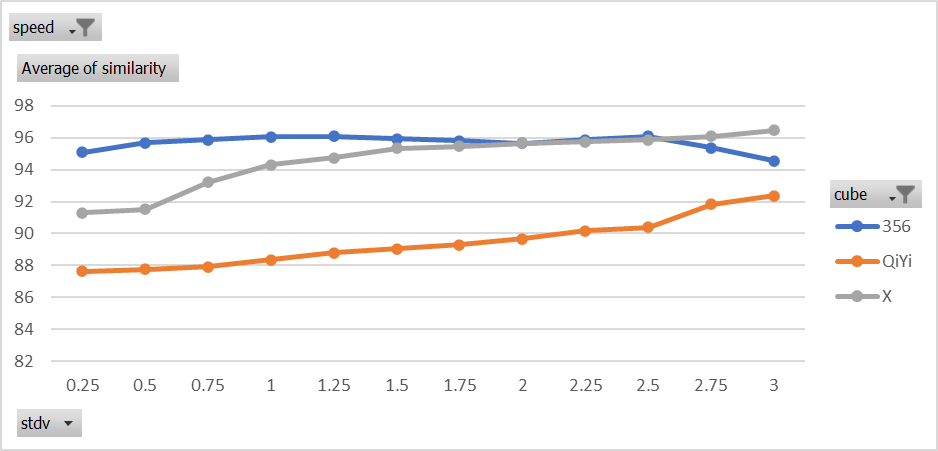
\includegraphics[width=0.75\linewidth]{Figures/7 Evaluation/similarity_by_cube_2tps.png}
\end{figure}

Basically the same as the overall average, just higher numbers overall.

\begin{figure}[h]
    \centering
    \caption{Average across 5 TPS}
    \label{fig:similarity-by-cube-5tps}
    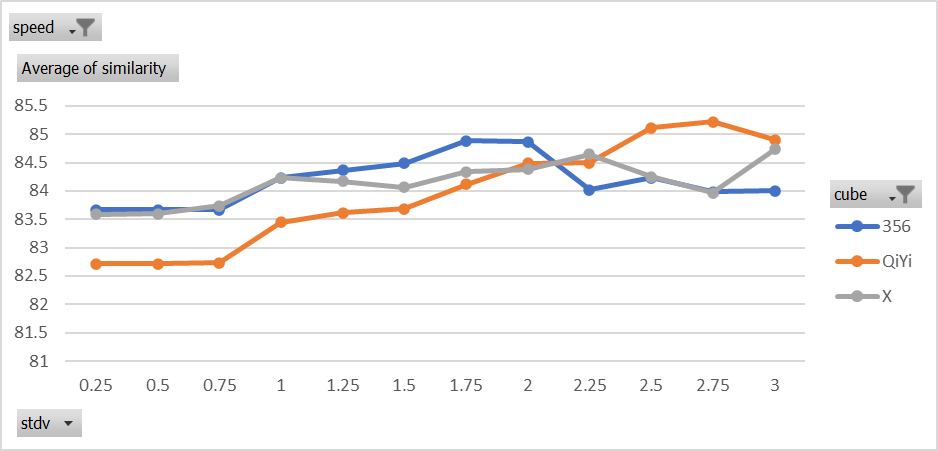
\includegraphics[width=0.75\linewidth]{Figures/7 Evaluation/similarity_by_cube_5tps.png}
\end{figure}

How is this for volatility? 

It's interesting that the 356 and the X start out virtually identical.
Also interesting is that the QiYi achieves the highest overall accuracy
of all three cubes.

\begin{figure}[h]
    \centering
    \caption{Effect of window size on accuracy of detection by cube}
    \label{fig:similarity-by-window-size}
    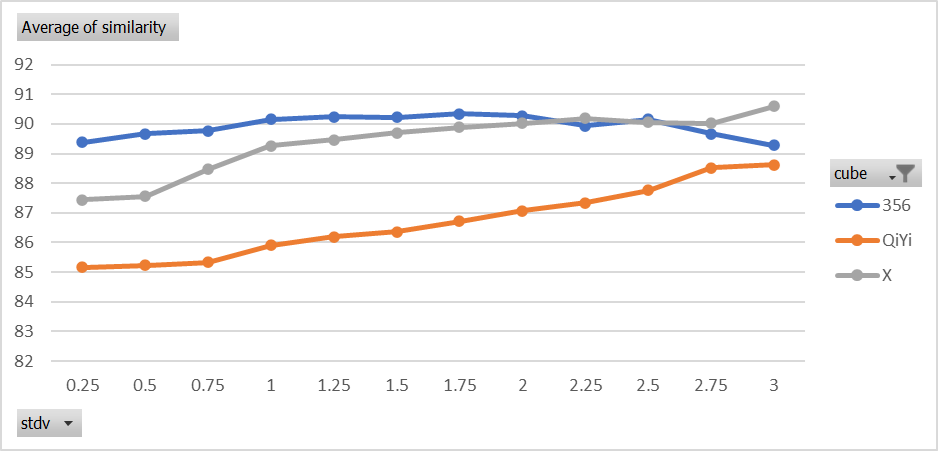
\includegraphics[width=0.75\linewidth]{Figures/7 Evaluation/similarity_by_cube.png}
\end{figure}

A higher window size consistently improved the accuracy of detection.
That said we do start seeing some decreases at a window size of 10, it
would be interesting to see when the window size starts inhibiting
accuracy.

I did not include the breakdown by speed because the graphs are
basically identical.

\begin{figure}[h]
    \centering
    \caption{Effect of alt\_min on accuracy of detection by cube}
    \label{fig:similarity-by-alt-min}
    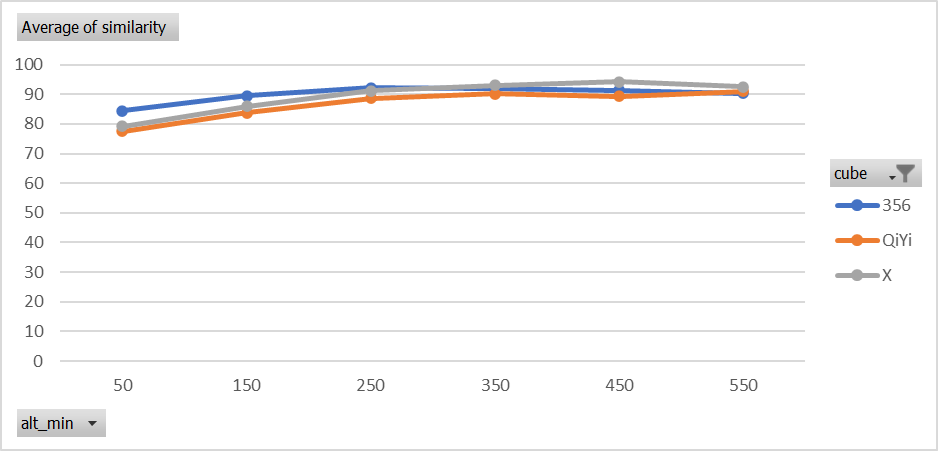
\includegraphics[width=0.75\linewidth]{Figures/7 Evaluation/similarity_by_alt_min.png}
\end{figure}

Like the window\_size, a higher alt\_min tends to correlate with a
higher accuracy; however, a low alt\_min doesn't hurt nearly as much as
a low window\_size.

\subsection{It is possible for all cubes to have a perfect accuracy}

\begin{figure}[h]
    \centering
    \caption{Best accuracy for each window\_size}
    \label{fig:max-similarity-by-window-size}
    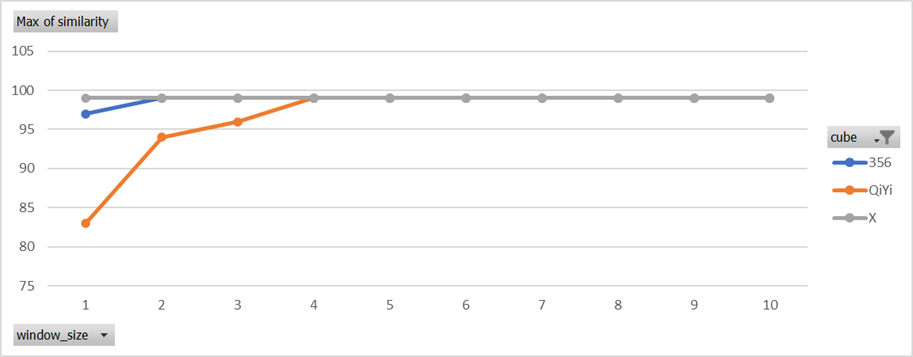
\includegraphics[width=0.75\linewidth]{Figures/7 Evaluation/max_similarity_by_window_size.png}
\end{figure}

\begin{figure}[h]
    \centering
    \caption{Best accuracy for each stdv multiplier}
    \label{fig:max-similarity-by-stdv}
    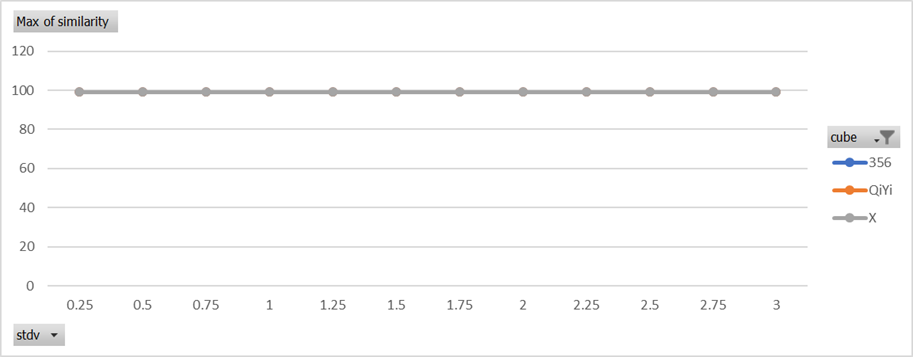
\includegraphics[width=0.75\linewidth]{Figures/7 Evaluation/max_similarity_by_stdv.png}
\end{figure}

\begin{figure}[h]
    \centering
    \caption{Best accuracy for each alt\_min}
    \label{fig:max-similarity-by-alt-min}
    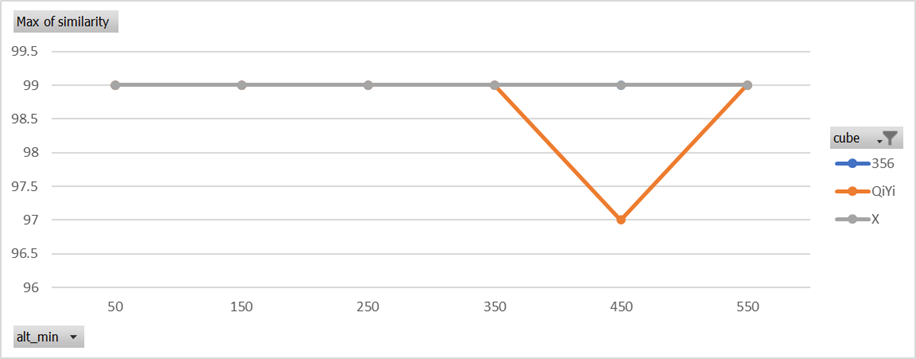
\includegraphics[width=0.75\linewidth]{Figures/7 Evaluation/max_similarity_by_alt_min.png}
\end{figure}

\subsection{Consistency of high accuracy}
Each cube underwent analysis for 1440 different parameter combinations.

\begin{figure}[h]
    \centering
    \caption{Total number of perfect detections by cube}
    \label{fig:perfect-detections-by-cube}
    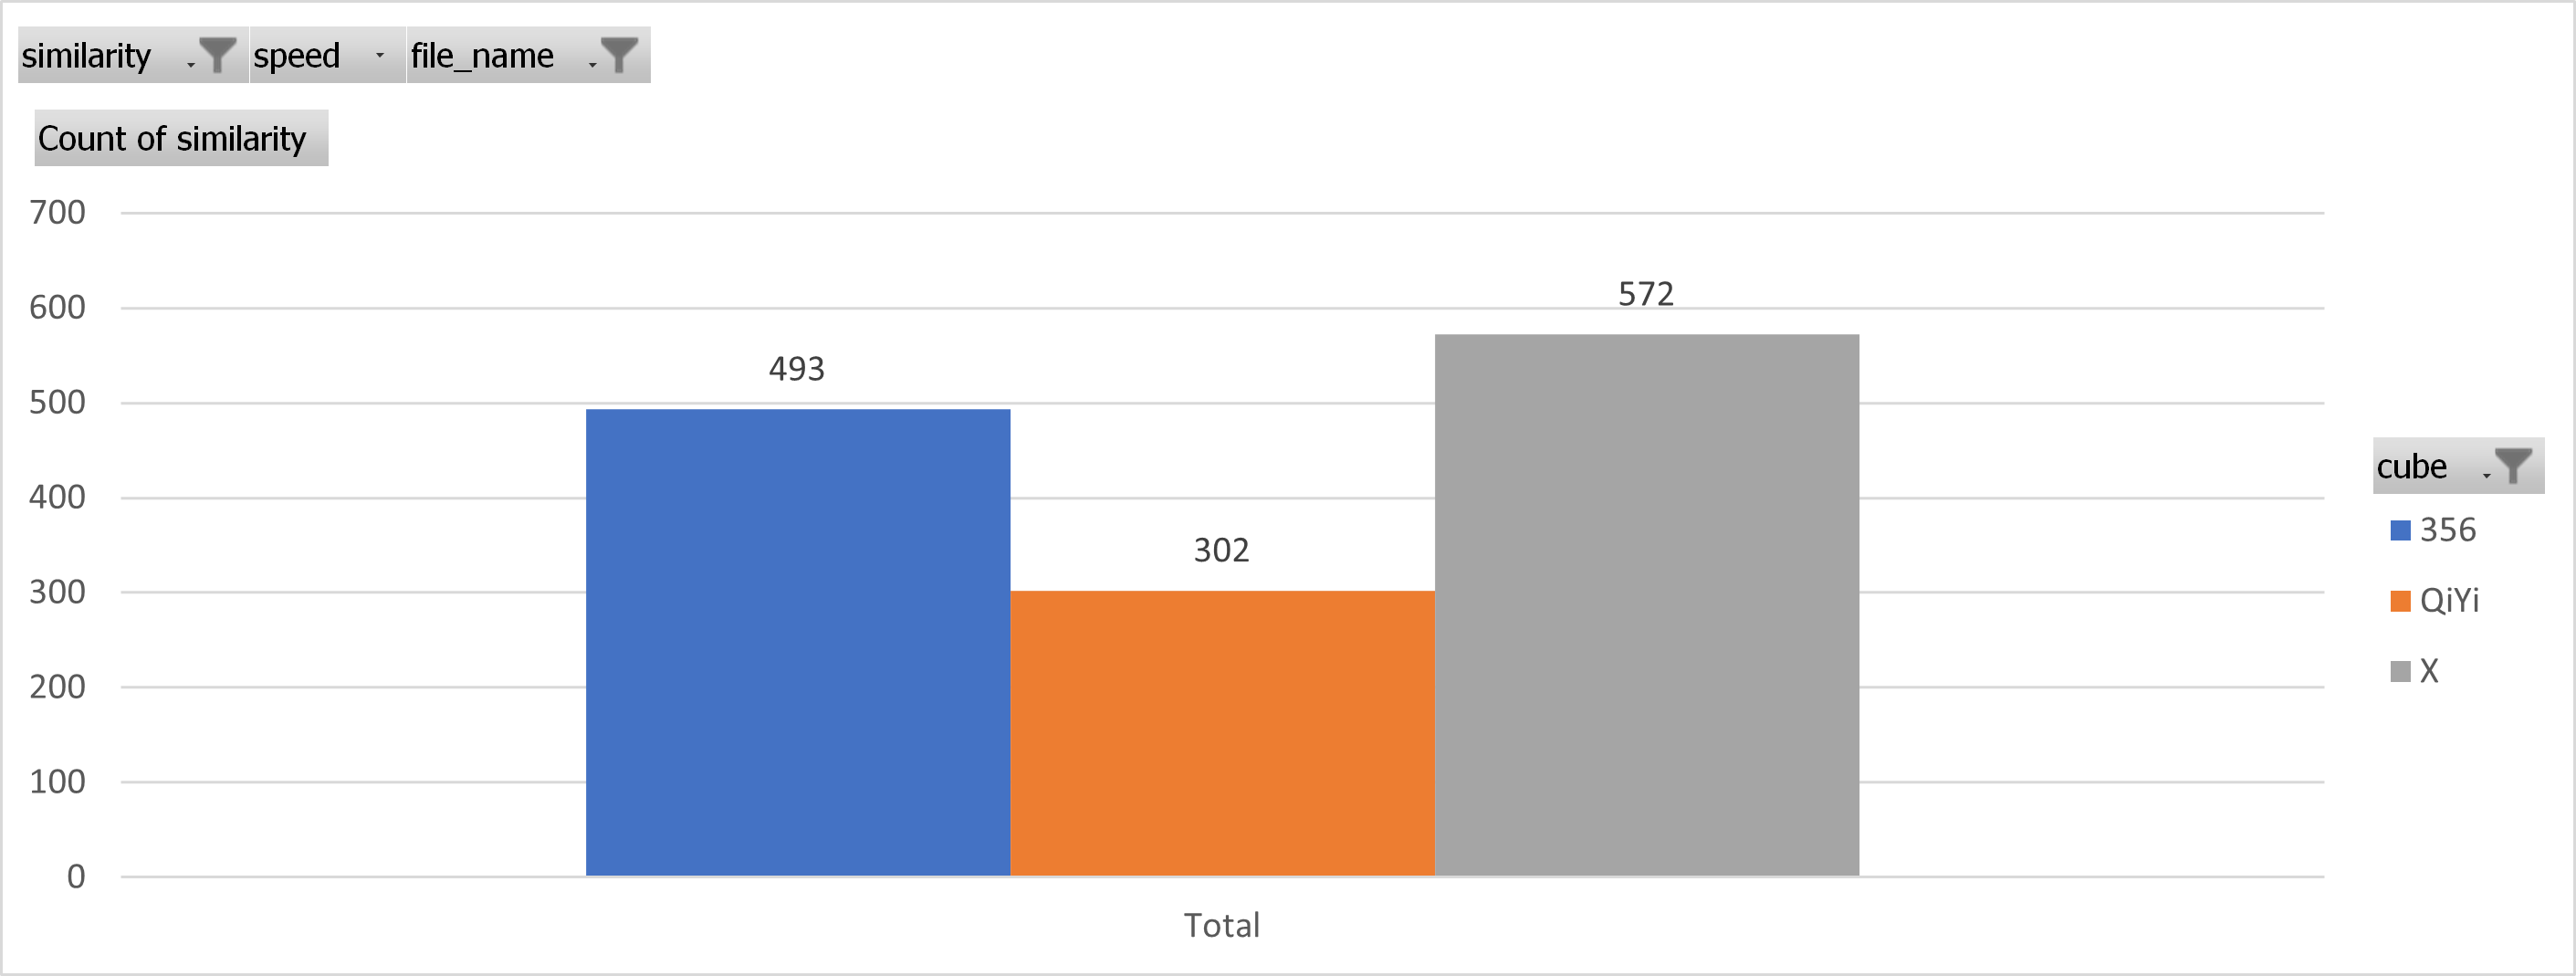
\includegraphics[width=0.75\linewidth]{Figures/7 Evaluation/perfect_detections_by_cube.png}
\end{figure}

\begin{figure}[h]
    \centering
    \caption{Total number of perfect detections by window\_size}
    \label{fig:perfect-detections-by-window-size}
    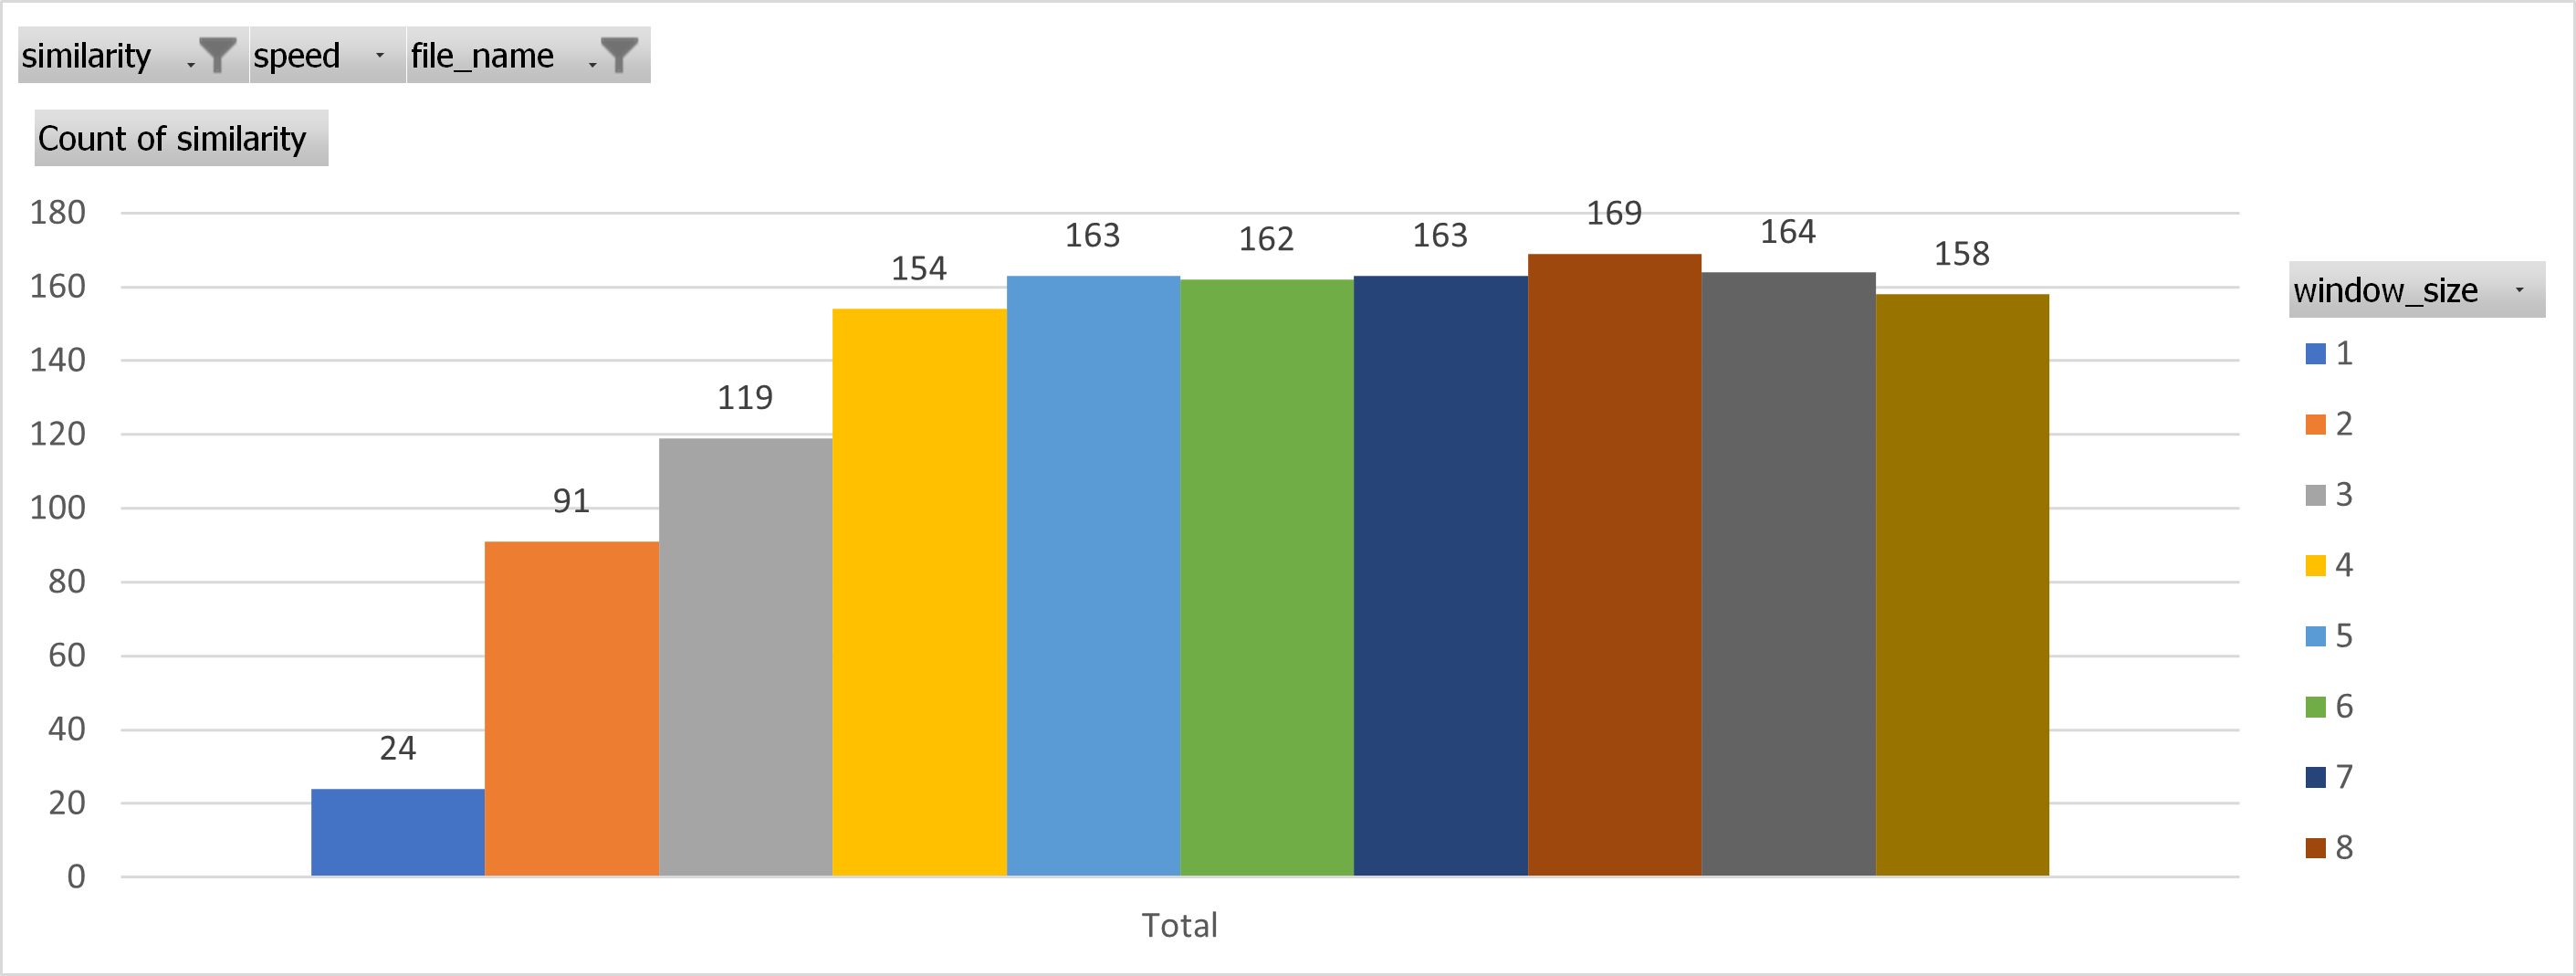
\includegraphics[width=0.75\linewidth]{Figures/7 Evaluation/perfect_detections_by_window_size.png}
\end{figure}

\begin{figure}[h]
    \centering
    \caption{Total number of perfect detections by stdv multiplier}
    \label{fig:perfect-detections-by-stdv}
    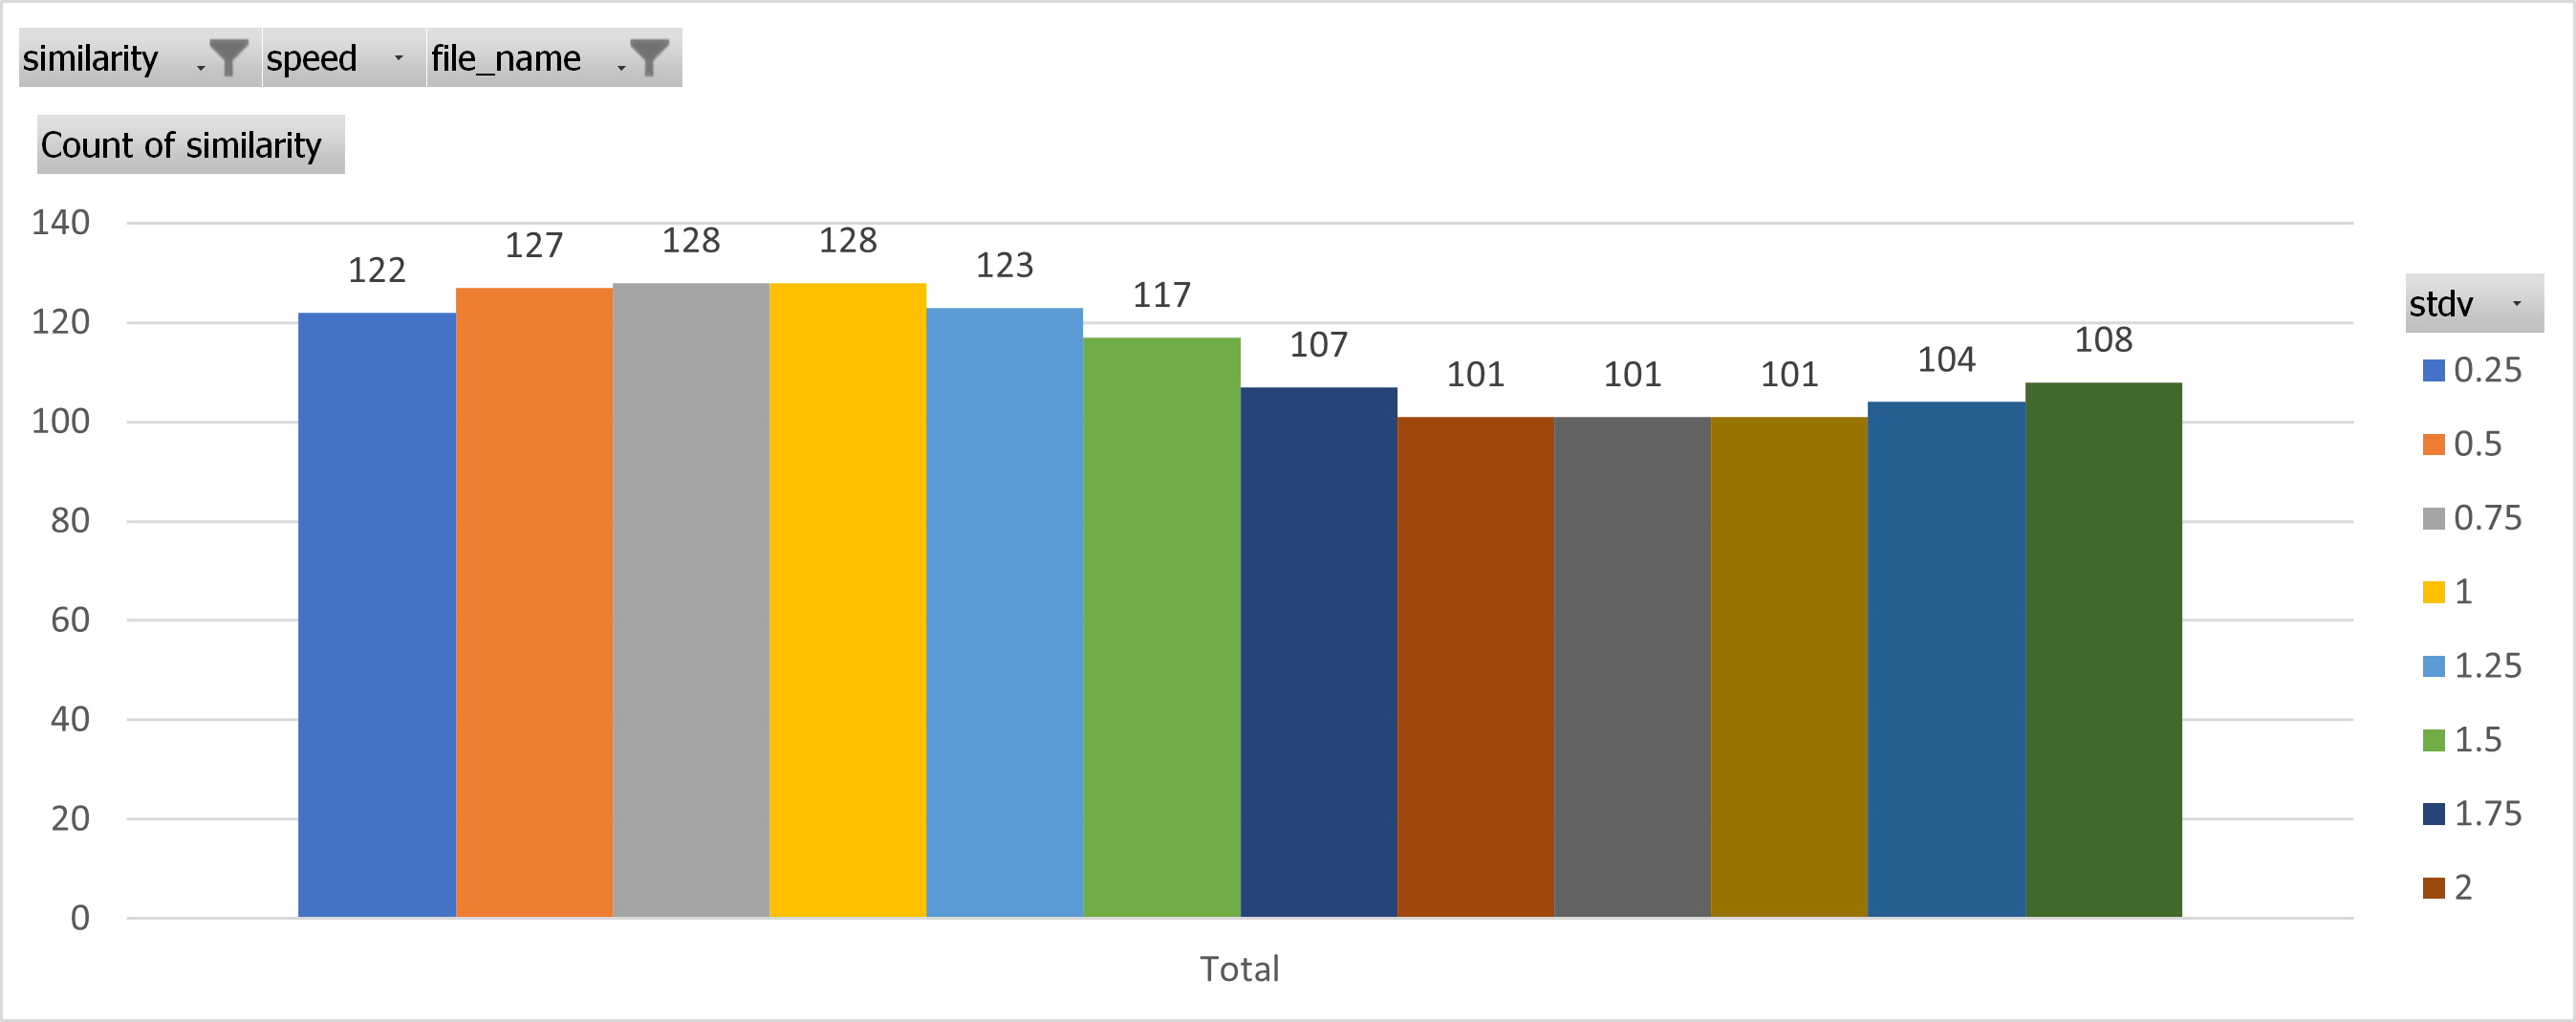
\includegraphics[width=0.75\linewidth]{Figures/7 Evaluation/perfect_detections_by_stdv.png}
\end{figure}

\begin{figure}[h]
    \centering
    \caption{Total number of perfect detections by alt\_min}
    \label{fig:perfect-detections-by-alt-min}
    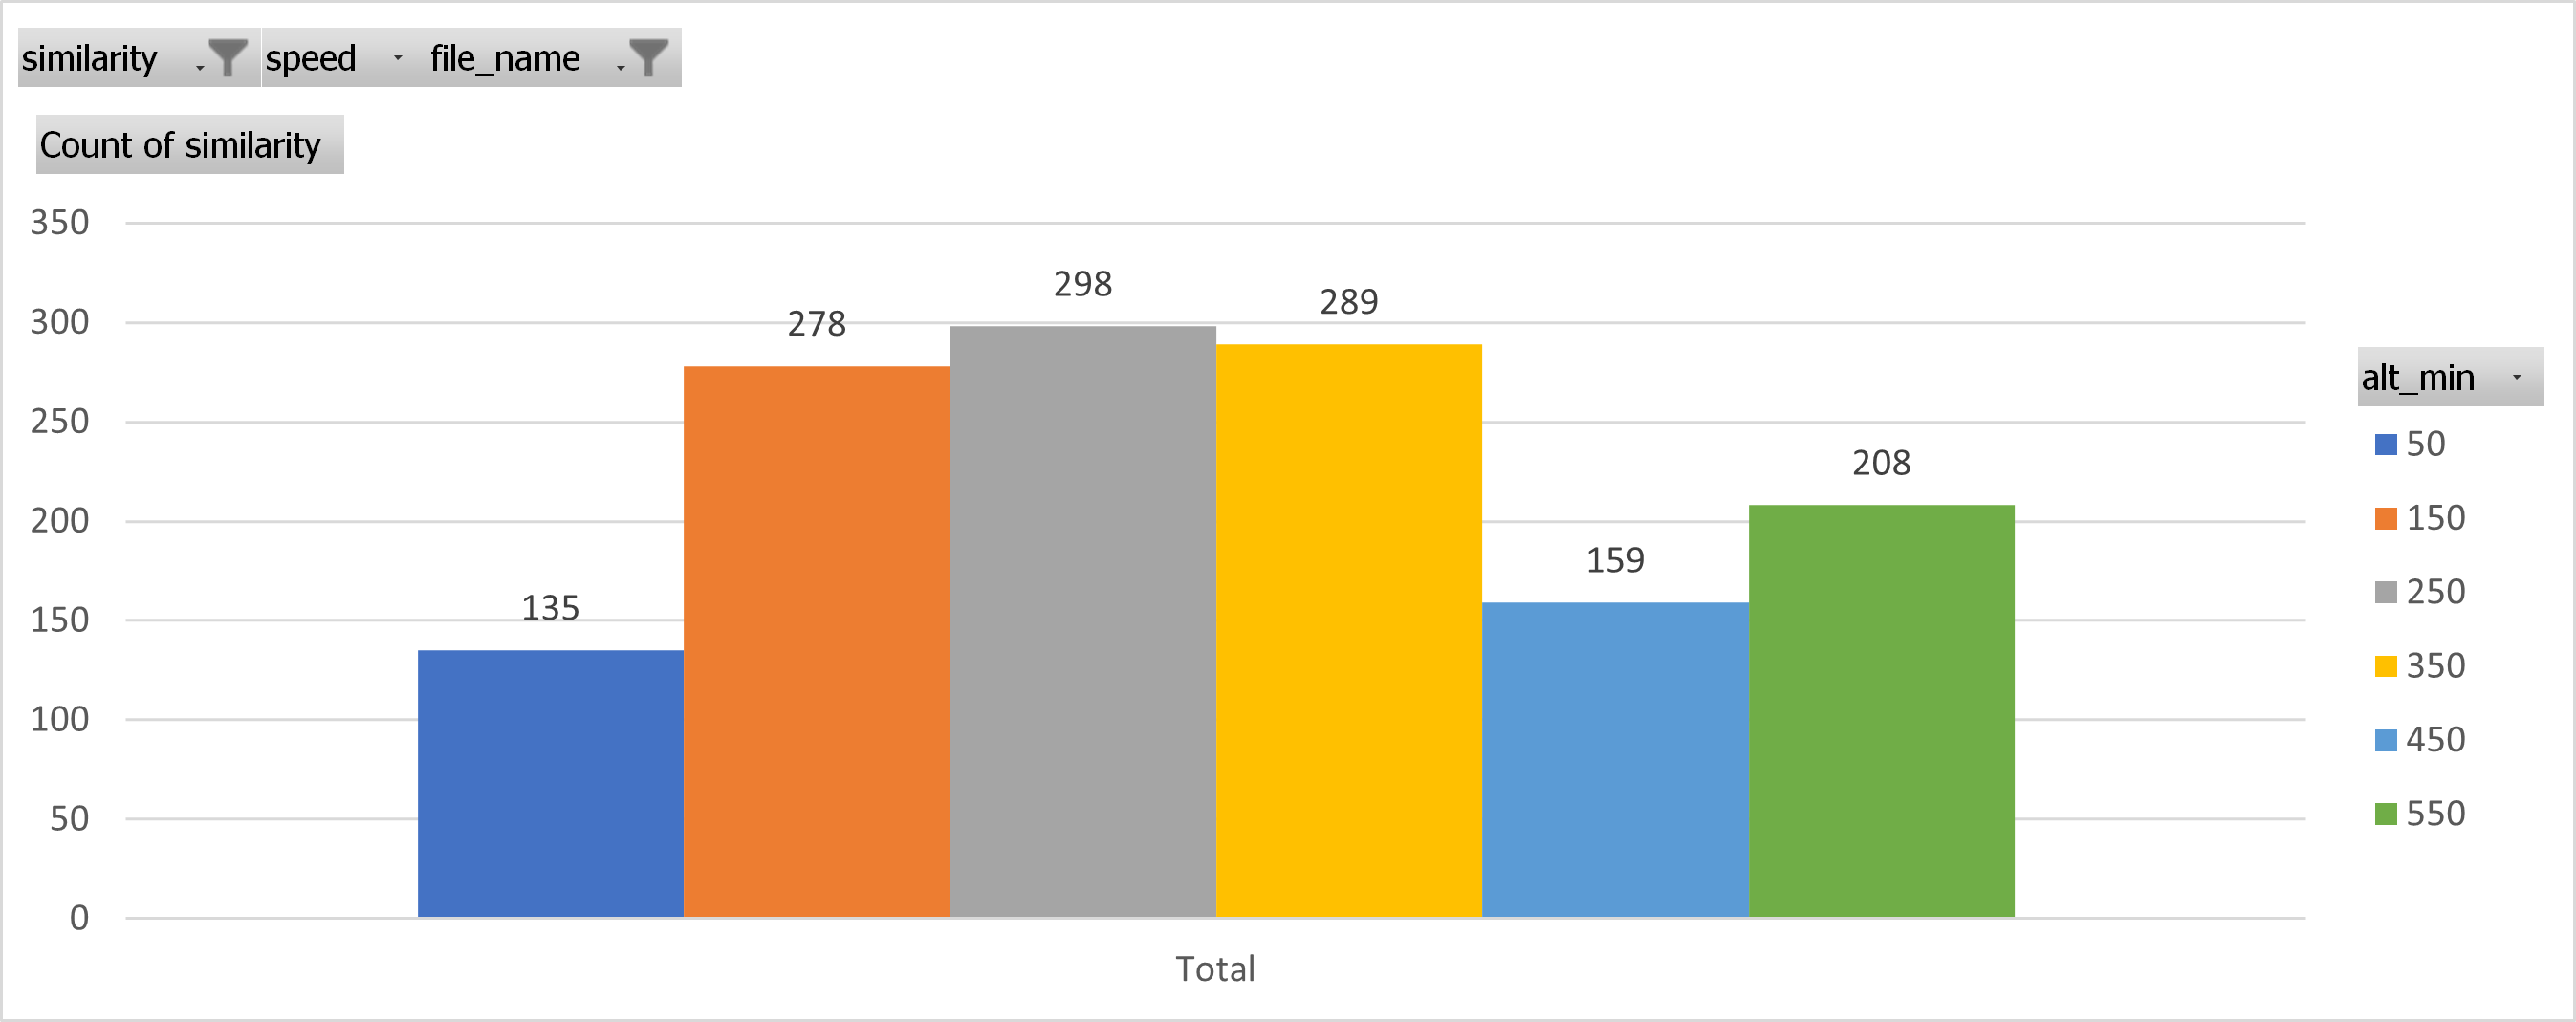
\includegraphics[width=0.75\linewidth]{Figures/7 Evaluation/perfect_detections_by_alt_min.png}
\end{figure}



\section{Move Tracking Granularity}

TODO discuss how well my design meets this requirement from the Introduction

The design must be capable of recording the time spent executing each individual face turn of a Rubik's Cube.


\section{Competition Legality}

TODO discuss how well my design meets this requirement from the Introduction

The design must be competition legal, meaning it results in a cube that either does not violate existing competition rules against the use of electronics or can be easily modified to regain compliance.

